\chapter{Background}\label{cha:background}
This chapter covers the main theoretical concepts underlying the problem domain and proposed solution.
Section~\ref{sec:back-pollen} gives a short overview of the current methods that are in use for pollen counting and the data that is available. Based on this, Section~\ref{sec:back-problem} formalizes the task as a machine learning problem.
A theoretical overview of the main building blocks of modern convolutional neural networks follows in Section~\ref{sec:back-cnn}, together with an overview of the metrics used to measure performance of object detection models in Section~\ref{sec:back-metrics}.
A basic understanding of the operation and components of a standard feed forward fully connected neural network is assumed for this section.

\section{Pollen Imaging}\label{sec:back-pollen}
There are two main methods of pollen analysis, image-based and non-image-based.
Non-image-based techniques employ a host of alternative sensing methods and will not be discussed further in this thesis.
Within the image-based methods there are two main imaging techniques.

\textit{Light microscopy} (LM) describes the method of observing a prepared sample with an optical microscope using visible light.
The sample is fixed to a translucent slide and is illuminated with a backlight.
It can either be observed through an eyepiece or photographed with a image sensor.
An example of a pollen grain is shown in Figure~\ref{fig:lm_and_sem}.
Because the grain is semi-translucent, differences in the surface texture can be observed, but only some areas are in focus.
A consequence of the high magnification is that the plane of focus is so narrow that only parts of the grain are in focus.

\begin{figure}[htb]
  \centering
  \begin{subfigure}[t]{0.4\textwidth}
    \centering
    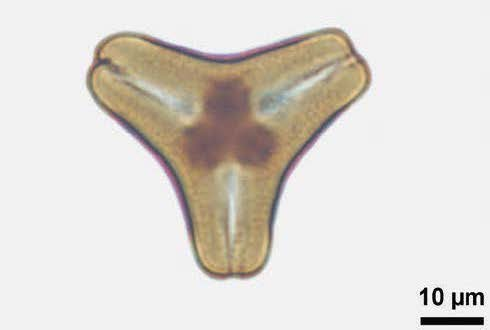
\includegraphics[width=\textwidth]{figs/background/pollen_lm.jpg}
    \caption{Light Microscopy}
  \end{subfigure}%
  \hspace*{0.04\textwidth}
  \begin{subfigure}[t]{0.4\textwidth}
    \centering
    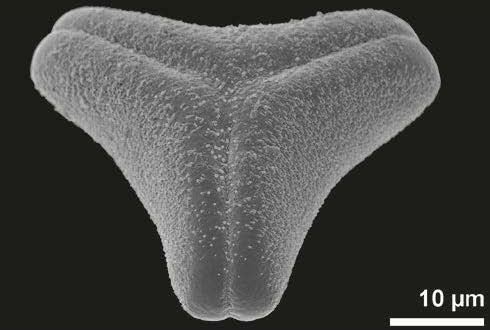
\includegraphics[width=\textwidth]{figs/background/pollen_sem.jpg}
    \caption{Scanning Electron Microscopy}
  \end{subfigure}
  \caption[Pollen grain imaging examples using LM and SEM]{\textit{Aetanthus coriaceus}.
  Imaged with LM (a) and SEM (b). \textcite[98]{halbritter_methods_2018} / cropped and rearranged, licensed under CC BY 4.0 URL\@: \url{https://creativecommons.org/licenses/by/4.0/}}\label{fig:lm_and_sem}
\end{figure}

\textit{Scanning electron microscopy} (SEM) is a very different approach where a focused beam of electrons is used to record the surface topology of a sample.
It captures very detailed features of the surface of the pollen grain but cannot reveal any of the substructure.
Because SEM imaging does not depend on focusing light, all parts of the image appear in focus and the resolution is much higher than what LM can achieve.
SEM imaging is however a more laborious process and requires more preparation of the sample.
SEM is also not suited for large samples where pollen grains must be observed over the entire slide.
This is the main reason why LM imaging is the only viable option when the task is to count pollen grains on a slide.

\section{Convolutional Neural Networks}\label{sec:back-cnn}
\emph{Convolutional Neural Networks} have been in active development for three decades and the umbrella of what the term encompasses continues to grow.
The basic concepts and building blocks have however remained quite unchanged since they were first used to predict handwritten digits in\ \textcite{1989Hdrw}.
An overview of the basic building blocks of a CNN will first be given, before expanding on each building block.
This section will also cover some of the newer concepts that have become commonplace additions to the basic model in later years.

A convolutional neural network consists of stacked, layered, operations.
There are two types of layers, \textit{convolutional}, and \textit{spatial pooling}.
The convolutional layers extract \textit{feature maps} by applying several trainable filters to the input, before applying a nonlinear activation function to the result.
The spatial pooling layers operate in a similar fashion by applying an operation to a receptive field which is moved over the input feature map.
The operation is designed to down sample the input, so the resulting feature map has reduced dimensions.
The two layers are stacked alternatingly, with the idea being that the complexity of the features extracted increases with the depth of the network.

\subsection{Convolution}

The central concept of the convolutional layer is the \textit{convolution operation}.
Let the kernel, \(w\), be a \(k\by k\) dimensional matrix.
This kernel will operate on the output of the preceding layer, \(x\).
The output from the convolution can be calculated as follows,

\[w\ast x_{ij}=\sum_{m}\sum_{n}  w_{mn}x_{i-m,j-n}\]

Where \((m,n)\) spans the index set of the kernel, which is center originated, i.e., \(w_{0,0}\) is the center element of the kernel.
The patch of \(x\) involved in the sum at each step is referred to as the \textit{receptive field}.
As the operation is repeated for every index of \(x\), the receptive field slides across the input.
The resulting output of the convolution is referred to as a \textit{feature map}.

\begin{figure}[htb]
  \centering
  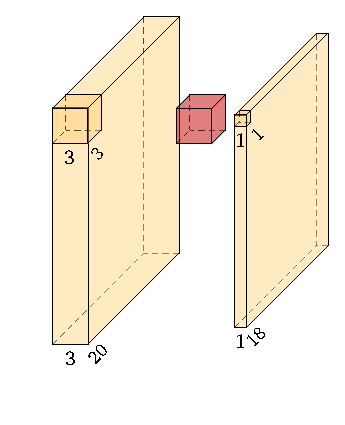
\includegraphics[width=0.4\textwidth]{figs/background/conv.pdf}
  \caption[Convolution operation]{Visualization of the convolution operation.
In red is a filter containing three \(3\by 3\) kernels.
The element wise multiplication between the filter and receptive field and subsequent summation produces a single scaler in the feature map.
The operation is repeated over the index set of the input, producing the complete feature map.
Visualization library \parencite{haris_2018}.}\label{fig:cnn}
\end{figure}

Usually, the input to a convolutional layer contains multiple channels, e.g.,\ an RGB input image which has three channels representing the separate red, green, and blue color channels.
To handle this, a stack of kernels is used, one for each input channel.
Each channel is convolved with its own kernel and the result is added together across the channels, which produces a single feature map.
An example of such a convolution operation is shown in Figure~\ref{fig:cnn}.
This stack of kernels is referred to as a \textit{filter}.
For a convolutional layer to produce \(N\) feature maps, \(N\) filters are needed.
It is common to increase the number of filters as the image is continually downsampled through the layers on the neural network.

At the edges of \(x\) the sum is undefined because the receptive field moves beyond the bounds of \(x\), causing a reduction in the size of the output.
This can be mitigated by \textit{padding} the input.
When the receptive field moves beyond the bounds of \(x\), a stand-in value is used instead.
This can be visualized as \textit{padding} the input with said value.
Zero is often used as the padding-value.

Dimensionality reduction is also possible using the concept of \textit{stride}, which refers to how the receptive field moves across the input relative to the index of the feature map.
In the base case, the receptive field moves by one step for every element in the feature map.
With an increased stride, the receptive field `jumps over' positions for every step in the feature map, thus shrinking its size.

One of the more important aspects of convolutions arises from the fact that the kernel is applied in the same way over the whole image.
This parameter sharing means that features are extracted from the input, regardless of their location\ \parencite{lecum1989}.
It also reduces the computational complexity involved in training the model.

Because convolution is a linear operation, non-linearity must be added if the network is to be able to approximate a non-linear function.
As with normal fully connected networks, this is achieved by applying an activation function to the feature map.
The same activation functions that are commonly used in fully connected networks are also used in CNNs.
Because of the depth of the models’ architectures in use today, the \textit{rectified linear unit} (ReLU), and its variations, are commonly used.

\subsection{Spatial pooling}
Even though the convolution operation extracts features wherever they exist within an image, a new problem arises when layers are stacked in order to extract higher level features from the combination of features below.
Local variations in the relative placement of features will have a big impact on later filters' ability to combine them and this would have to be accounted for by dramatically increasing the number of filters.\ \textcite{lecun1998gradient} presents a simple solution to this problem with a \textit{sub-sampling} layer, referred to as a \textit{pooling} layer today, which reduces the dimensions of the feature map by applying a local pooling function, similarly to the convolution operation.
Common pooling functions are maximum and average.
The pooling operation is applied to each channel separately so only the width and height is downsampled.
Pooling retains the relative placement of features within the image but allows the network to ignore smaller variations in the relative configuration of features across all the channels of the feature map.

\subsection{Cross channel pooling}

As mentioned, it in customary to increase the depth of the feature maps as they get downsampled throughout the network.
This is necessary if the model is to learn more complex features that may require many layers to be represented in full.
Combining information from multiple channels could be helpful in building more rich feature maps.
This is the proposal in\ \textcite{lin2014network}.
To enhance model discriminability, they emulate a fully connected layer working across the channels by using a convolutional layer with a \(1\by 1\) kernel.
This effectively creates connections between local features across the channels of the feature maps, allowing the feature map to be projected into a map with a different depth.

The primary motivation for using this technique today is to lower the computational cost of standard convolutions by reducing the depth of the input prior to a larger convolution.
The technique is now commonplace and featured in all deep CNN architectures.

\subsection{Batch normalization}
As the network trains, the parameters in each layer change, this causes the distribution of each layer’s output to shift.
As the distribution from previous layers change, this shift is propagated though to the layers downstream, and so each layer must deal with ever changing input distributions.
To overcome this, lower learning rates and careful parameter initialization is required.

A much more effective solution has been proposed by\ \textcite{ioffe2015batch} called \textit{Batch Normalization} (BN).
The proposed solution for convolutional networks is to normalize the output of each convolutional layer by first standardizing each feature dimension by the sample mean and sample variance across the current mini batch, then transforming each layer by a linear transformation with trainable parameters.
The linear transformation allows the network to restore the representative power of the layer after standardization.
By allowing the filters to only focus on learning features, instead of having to adapt to constantly shifting inputs, training is accelerated which allows for higher learning rates.

{\it\color{red}
Perchance i could interest thee in some transfer learning
}

\section{Metrics}\label{sec:back-metrics}
An important step towards building a model is defining how to measure its performance.
Implicitly, this is done through the construction of a \textit{Loss function}.
The models examined in this thesis do not employ novel Loss functions, so delving into their construction is not warranted.
The metrics used when measuring the performance of object detectors, specifically, are however of interest.

\subsection{Precision and recall}
The precision and recall of a model refer to its ability to correctly locate and label the objects within an image.
Before defining precision and recall, the following quantities must be introduced,

\begin{center}
  {\setlength{\fboxsep}{1em}
  \fbox{%
  \begin{minipage}{0.9\textwidth}
  {\bf True Positive (TP):} Number of objects correctly located and labelled.\\[1ex]
  {\bf False Positive (FP):} Number of incorrect predictions.\\[1ex]
  {\bf True Negative (TN):} Correct non-prediction, not usually relevant.\\[1ex]
  {\bf False Negative (FN):} Number of objects missed by model.
  \end{minipage}}}
\end{center}

Precision measures the accuracy of the model, i.e.,~how many of the positive predictions are correct.
Recall measures how many of the positive instances the model correctly labels.
They are computed from the above quantities as follows,

\begin{align*}
  \text{\bf precision}=\frac{TP}{TP+FP}\\[1em]
  \text{\bf recall}=\frac{TP}{TP+FN}
\end{align*}

These two metrics are the basis for how all object detection models are evaluated and there is usually a tradeoff between the two, e.g.\ a model can have very high recall, meaning if correctly identifies most of the potential objects, but if it also identifies many other non-objects the precision is reduced.
Inversely a model could be very certain that it returns correctly identified objects, at the cost of ignoring objects it is not to sure about.

A popular accuracy measure which derives from the precision and recall values is the \(F_1\) score, it may also be referred to as the dice score.
It is defined as follows,
%
\begin{align*}
  F_1=2\frac{\text{precision}\cdot\text{recall}}{\text{precision}+\text{recall}}
\end{align*}

The \(F_1\) score measures the balance between precision and recall values and is useful in cases where both measures are \textit{equally} important performance indicators.

\subsection{Intersection over union}
Precision and recall form the basis for how all object detection models are evaluated, but the definitions are not complete without a definition of what constitutes a \textit{correct} prediction.
Correctness is commonly defined using the \textit{intersection over union} (IoU) between the predictions and ground truths.
IoU measures the overlap between two boundaries.
As the name indicates, it is defined as the ratio between the intersection and union of the boundaries,

\begin{figure}[htb]
  \centering
  \begin{gather*}
    \text{IoU}=\frac{\text{area of intersection}}{\text{area of union}}
  \end{gather*}
  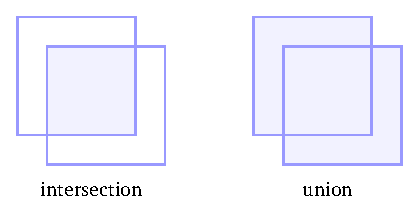
\includegraphics[width=0.55\textwidth]{figs/background/iou.pdf}
\caption[Intersection over union]{Visualization of the intersection over union of two boundaries.
The named region is shaded.}\label{fig:iou}
\end{figure}

The definition what is considered as a correct prediction (TP) can then be defined.
Given prediction \(\hat{X}\) with label \(\hat{X}_l\) and bounding box \(\hat{X}_u\). \(\hat{X}\) is considered a True Positive if there exists a ground truth \(Y\), where \(Y_{l}=\hat{X}_l\) and \(\text{IoU}(\hat{X}_u, Y_{u})\ge \mu \).
Where \( \mu \) is some threshold value, often 0.5.

\subsection{Mean average precision}
Mean average precision (mAP) is a popular metric for measuring the performance of object detection models.
It is computed by taking the mean of the \textit{average precision} values for each class.

From a list of all detections made for a class, ranked in ascending order of confidence, a precision-recall curve is drawn.
This shows how precision changes as recall rises over the range [0,1] as more and more detections from the ranked list are included in the precision/recall calculations.
The AP describes the shape of the precision-recall curve, and can be calculated a few different ways.
This thesis will use the definition of AP specified in the evaluation procedure for the VOC2007 image detection challenge.
For convenience, the definition of AP, as given in\ \textcite{everingham2010pascal} is repeated bellow.

AP is measured by taking the mean of precision values taken at 11 evenly spaced recall values as follows,

\begin{equation}\label{eq:average-precision}
  AP=\frac{1}{11} \sum_{r\in \{0,0.1,\dots,1\}}p_{interp}(r)
\end{equation}

Because the precision-recall curve often times is quite erratic, the precision value at a given recall level, \(r\), is interpolated by finding the maximum precision value at any recall level exceeding \(r\),

\begin{equation*}
  p_{interp}(r)=\max_{\tilde{r}:\tilde{r}\geq r}p(\tilde{r})
\end{equation*}

This section has detailed the current methods employed for automated pollen counting, as well as the foundational building blocks of a CNN\@.
Most research and application of CNN based methods is in regard to classification, which only solves part of the problem of counting pollen.
To fully automate the task, a subcategory of deep CNNs capable of predicting both classes and locations is required.
The next chapter will detail how \textit{object detection} can be solved using a CNN by detailing how they have been used to solve tasks similar to pollen counting.
The available literature relating to other attempts at solving the problem of counting pollen will also be given.
